\providecommand{\pgfsyspdfmark}[3]{}
\providecommand{\savepicturepage}[3]{}

\documentclass[11pt,letterpaper]{article}
\usepackage[lmargin=1in,rmargin=1in,tmargin=1in,bmargin=1in]{geometry}

% -------------------
% Packages
% -------------------
\usepackage{
	amsmath,			% Math Environments
	amssymb,			% Extended Symbols
	enumerate,		    % Enumerate Environments
	graphicx,			% Include Images
	lastpage,			% Reference Lastpage
	multicol,			% Use Multi-columns
	multirow,			% Use Multi-rows
	gensymb
}


% -------------------
% Font
% -------------------
\usepackage[T1]{fontenc}
\usepackage{charter}
\usepackage{xcolor}

% -------------------
% Commands
% -------------------

\newcommand{\prob}{\noindent\textbf{Problem. }}
\newcounter{problem}
\newcommand{\problem}{
	\stepcounter{problem}%
	\noindent \textbf{Problem \theproblem. }%
}
\newcommand{\answer}{\noindent \textbf{Answer. }}
\newcommand{\pspace}{\par\vspace{\baselineskip}}
\newcommand{\ds}{\displaystyle}


% -------------------
% Header & Footer
% -------------------
\usepackage{fancyhdr}

\fancypagestyle{pages}{
	%Headers
	\fancyhead[L]{}
	\fancyhead[C]{}
	\fancyhead[R]{}
\renewcommand{\headrulewidth}{0pt}
	%Footers
	\fancyfoot[L]{}
	\fancyfoot[C]{}
	\fancyfoot[R]{}
\renewcommand{\footrulewidth}{0.0pt}
}
\headheight=0pt
\footskip=14pt

\pagestyle{pages}


% -------------------
% Content
% -------------------
\begin{document}
\noindent\textbf{\large Calculus I (AM\_\_1050AH / MSF\_10110) \\ 2022 Fall \\ Application of Derivatives (5.3-5.4) (Answer Key)}

\bigskip

\noindent Note that in problems for related rates, you should clearly indicate the unit of your answer. 
\bigskip

\problem A 2-meter ladder leaning on the up-straight wall is sliding off the wall.  Currently, the height of the ladder tip is 1.7 meters and the foot of the ladder is moving away from the base of the wall at a speed of 17 centimeters / seconds.  How fast is the (acute) angle between the ladder and the ground decreasing now? \vspace{6mm}

\answer 

\begin{figure}[h]
    \centering
    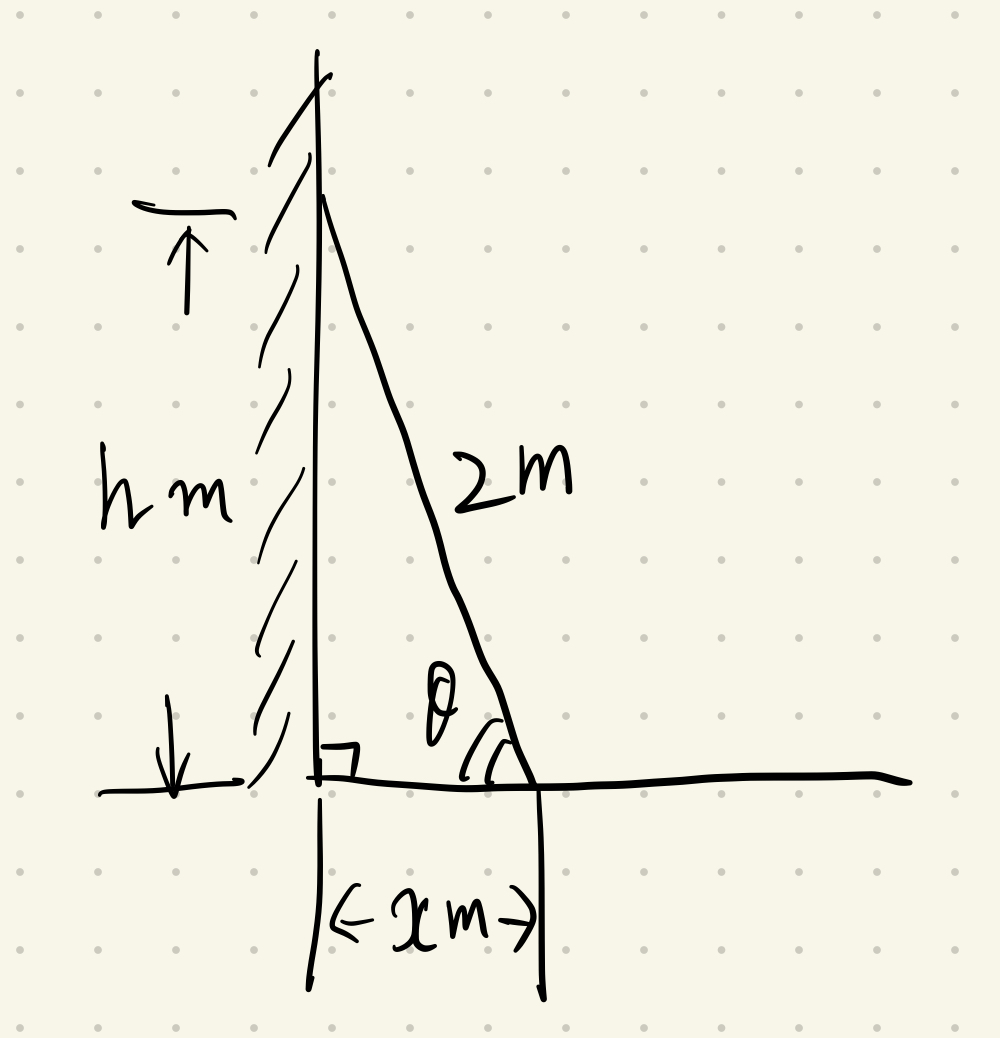
\includegraphics[width = 0.25\textwidth]{../graph/A12_Sol_1.png}
\end{figure}

\noindent As shown in the figure above, denote the acute angle between the ladder and the ground as $\theta$ (in radians), the distance between the ladder foot and the base of the wall as $x$ (in meters), the height of the ladder tip as $h$ (in meters).  Then we have, from basic trigonometry:
\[x = 2\cos \theta\]
Differentiating both side by time $t$ (in seconds) and denoting $()'$ as differentiation by $t$, we have
\[x' = (2\cos\theta)' = -2\sin\theta\cdot\theta' = -h\theta' \]
where the second equality comes from chain rule differentiating first on $\theta$, and the second equality comes from basic trigonometry.  Since currently the ladder tip is $1.7$ meters tall, we have $h = 1.7$.  Also, the ladder foot is moving away from the base of the wall at a speed of $17$ cm/sec, so we have $x' = 0.17$ (note the units!).  Therefore, we have
\[\theta' = -\frac{x'}{h} = -\frac{0.17}{1.7} = -0.1\]
That is, the angle is \textit{decreasing} at a speed of $0.1$ radians per second.\vspace{6mm}

\newpage

\problem A rat is resting at the base of a 3-meter lamppost, while an owl flying with height 1.5 meters and 2 meters away from the rat is directly charging toward the rat at the speed of 0.5 meters / sec, as shown below.  What is the speed of the owl's shadow on the ground moving now? \vspace{6mm}

\begin{center}
    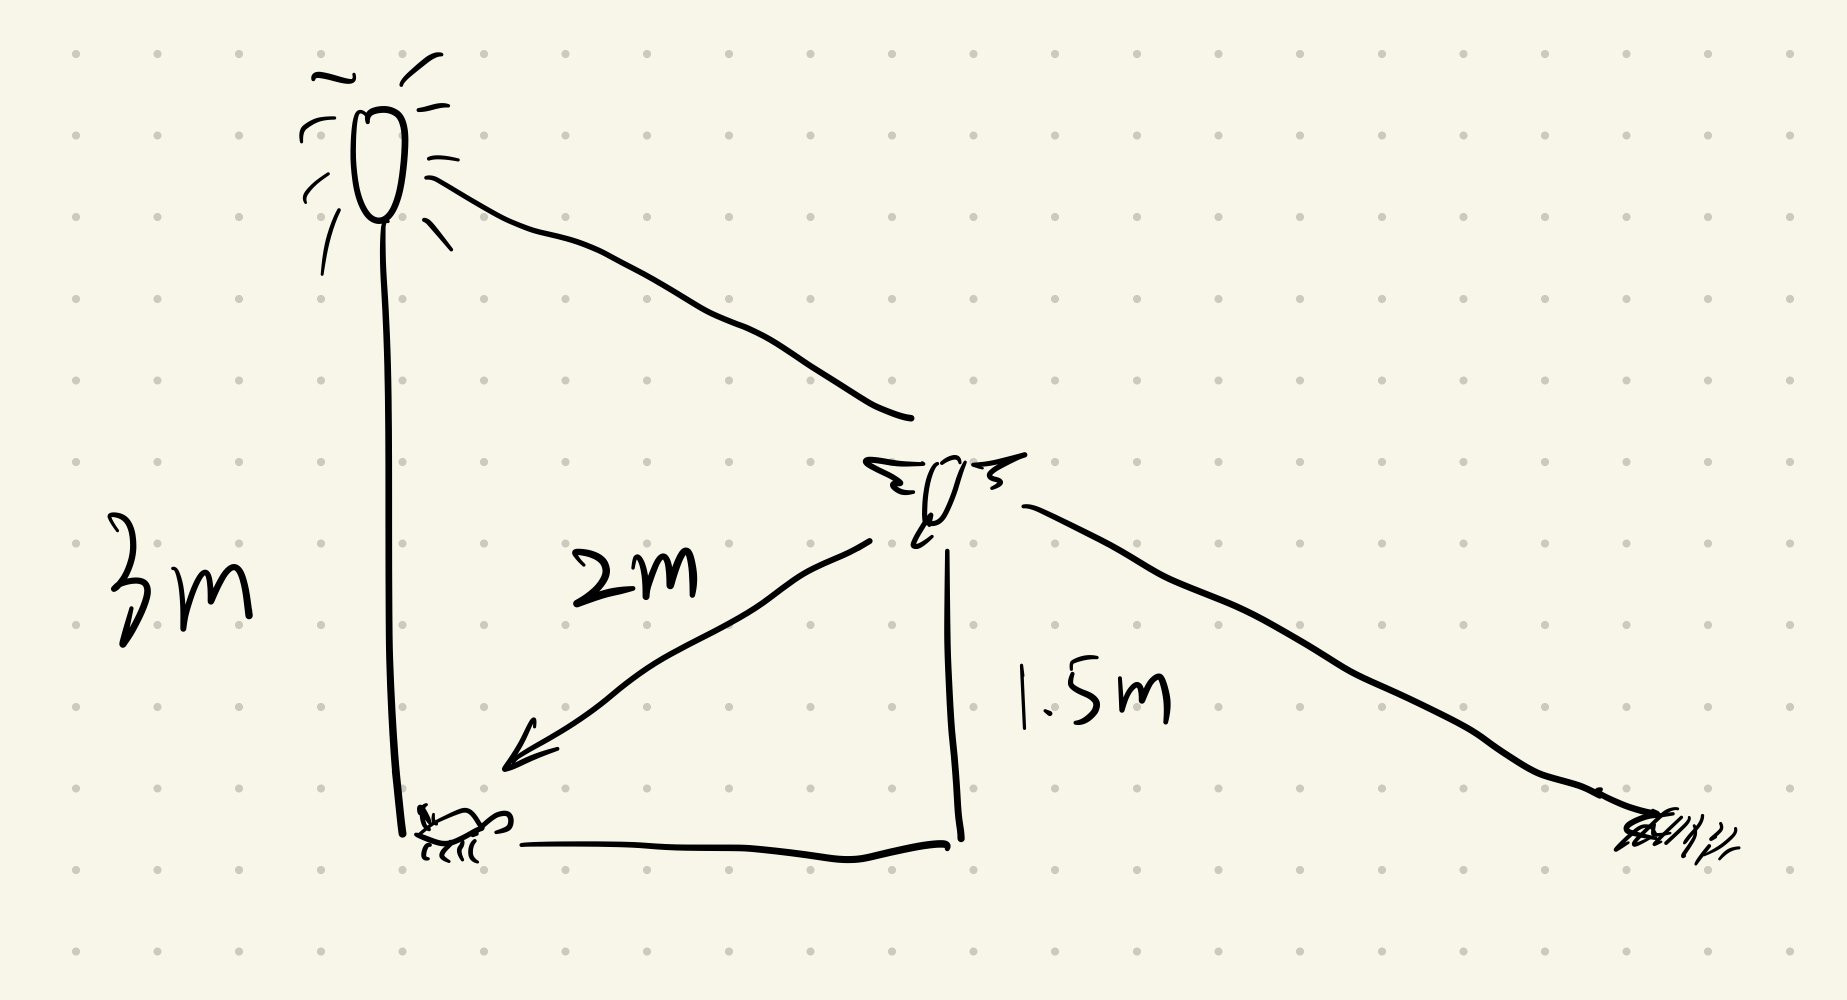
\includegraphics[width = 0.5\textwidth]{../graph/A12.png}
\end{center}

\answer
\begin{figure}[h]
    \centering
    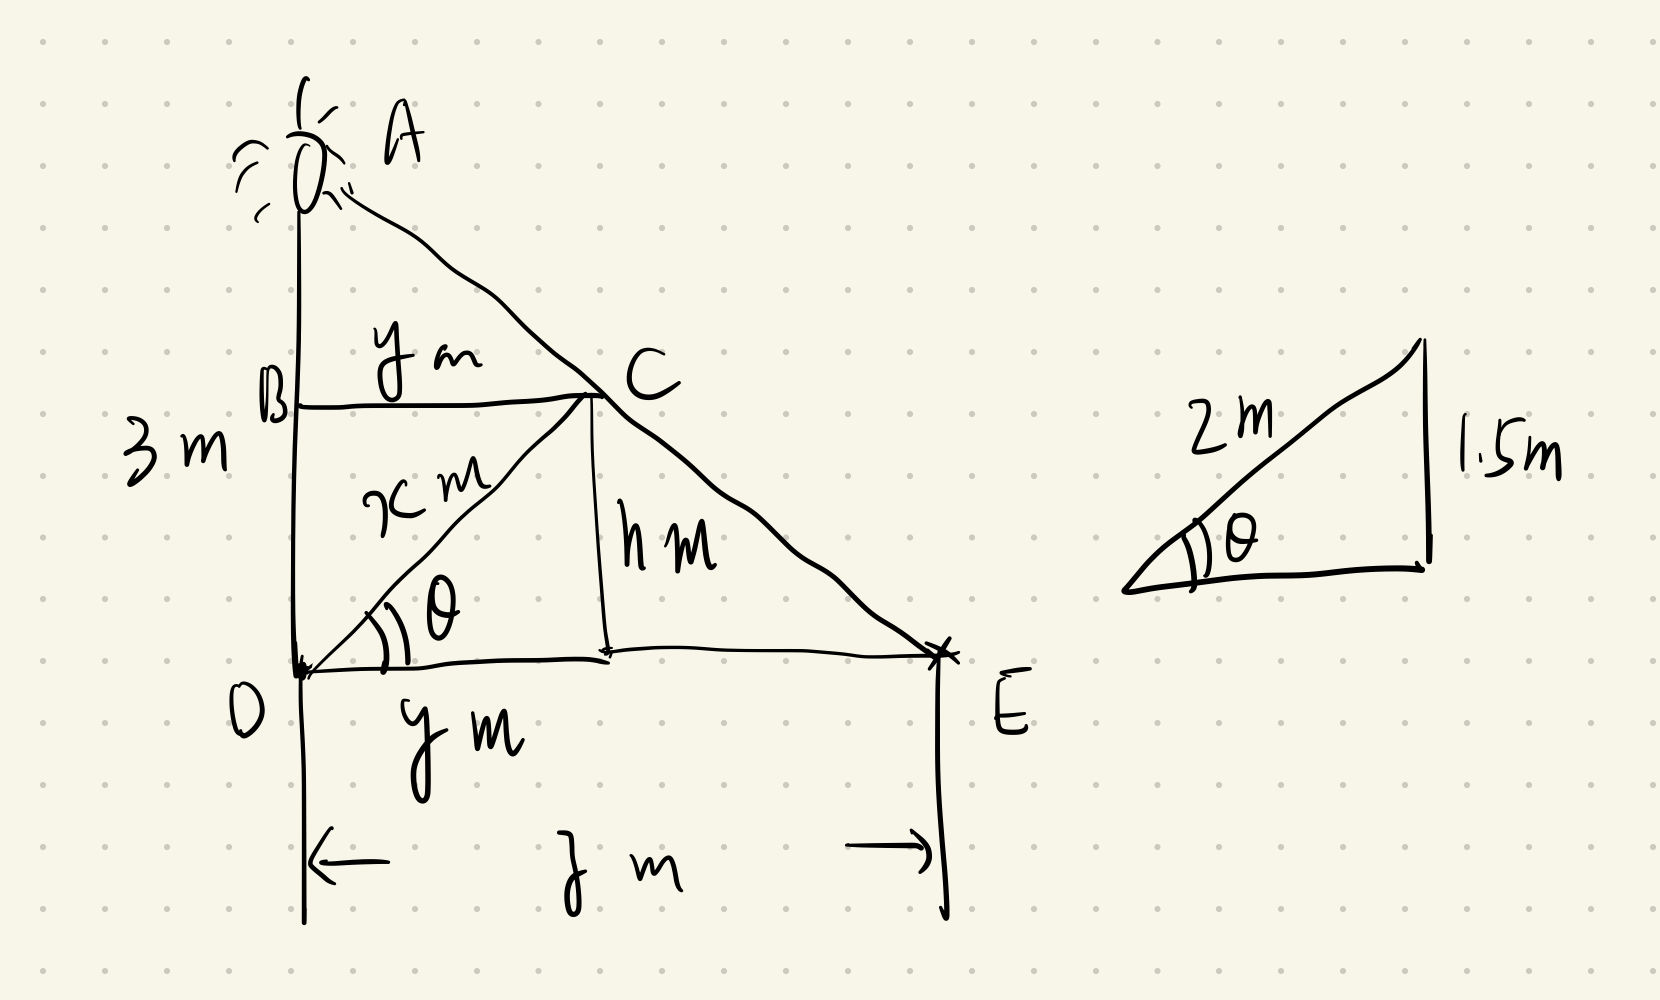
\includegraphics[width = 0.6\textwidth]{../graph/A12_Sol_2.png}
\end{figure}

\noindent As shown in the figure above, denote the distance between the owl and the rat as $x$ (meters), the height of the owl as $h$ (meters), the distance between the owl and the lamppost as $y$ (meters), and the distance between the owl's shadow and the rat as $z$ (meters).  Since the owl is charging straight toward the rat, its diving angle remains the same throughout the flight, which is denoted as $\theta$ in the figure.  From the initial position given by the problem, we yield
\[\sin \theta = \frac{1.5}{2} = \frac{3}{4} \qquad \cos \theta = \sqrt{1-\sin^2\theta} = \sqrt{1-\Big(\frac{3}{4}\Big)^2} = \frac{\sqrt{7}}{4}\]
Therefore, we can express $h$ and $y$ with $x$
\[h = x\sin \theta = \frac{3}{4}x \qquad y = x \cos \theta = \frac{\sqrt{7}}{4}x\]
Now using the similarity of $\bigtriangleup ABC$ and $\bigtriangleup ADE$, we yield
\[\frac{z}{3} = \frac{y}{3-h} \quad \Rightarrow \quad z = \frac{3y}{3-h} = \frac{3\cdot \frac{\sqrt{7}}{4}x}{3-\frac{3}{4}x} = \frac{\sqrt{7}x}{4-x}\]
Differentiating both sides by time $t$ (in seconds) and denoting $()'$ as differentiation by $t$, we yield:
\[z' = \Big(\frac{\sqrt{7}x}{4-x}\Big)' = \frac{\sqrt{7}(4-x) - \sqrt{7}x(-1)}{(4-x)^2}x' = \frac{4\sqrt{7}}{(4-x)^2}x'\]
Since currently the owl is $2$ meters away from the rat and is charging at a speed of $0.5$ meters per second, we have $x = 2$ and $x' = 0.5$. Therefore,
\[z' = \frac{4\sqrt{7}}{(4-2)^2}\cdot 0.5 = \frac{\sqrt{7}}{2}\]
That is, the shadow of the owl is moving at a speed of $\frac{\sqrt{7}}{2}$ meters per second. \vspace{6mm}

\newpage

\problem Sketch the function $f(x) = x^2e^{-x}$ including information from its first derivatives\vspace{6mm}

\answer The sketch is as follows, which originates from the steps laid out in the handout.
\begin{figure}[h]
    \centering
    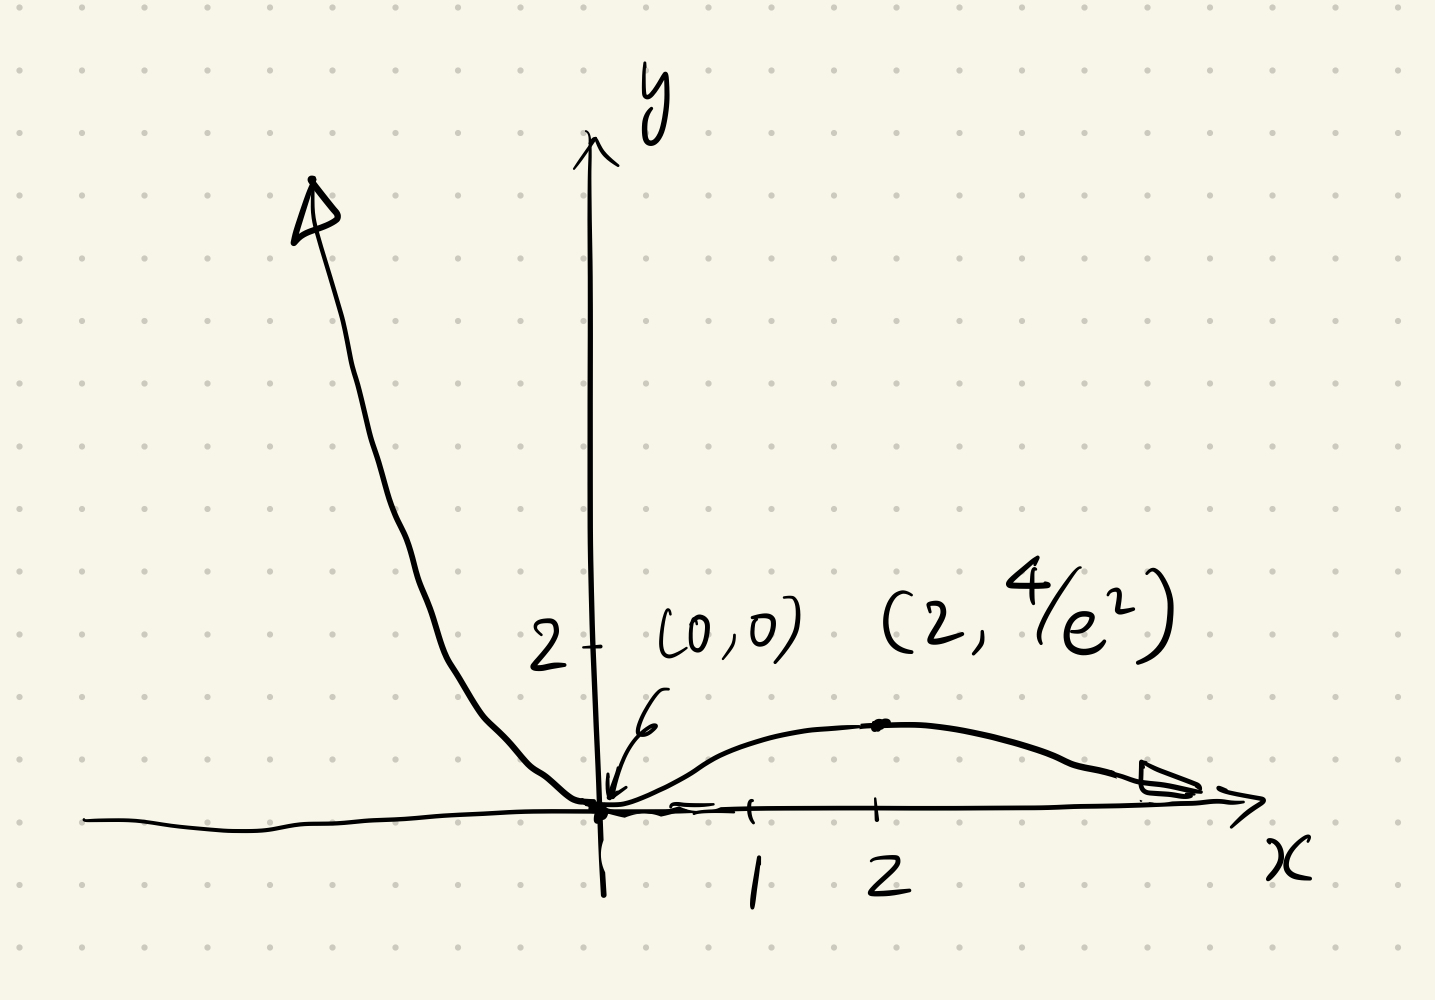
\includegraphics[width = 0.5\textwidth]{../graph/A12_Sol_3.png}
\end{figure}

\begin{enumerate}
    \item \textit{Domain and behavior at boundaries}: The domain of $f(x)$ is $(-\infty, \infty)$ since we may plug in any real number into $f(x)$.  To investigate the behavior of $f(x)$ when $x$ is approaching the boundaries $\pm \infty$, we evaluate the following limits:
    \[\lim_{x\rightarrow-\infty} x^2e^{-x} = \infty \cdot \infty = \infty\]
    \[\lim_{x\rightarrow\infty} x^2e^{-x} = \lim_{x\rightarrow\infty} \frac{x^2}{e^{x}} = \lim_{x\rightarrow\infty} \frac{2x}{e^{x}} = \lim_{x\rightarrow\infty} \frac{2}{e^{x}} = \frac{2}{\infty} = 0\]
    where in the latter limit we transformed a $\infty \cdot 0$ indeterminate form into $\frac{\infty}{\infty}$ and repeatedly used L'Hôpital's rule.  Therefore, $f(x)$ tends to $0$ when $x$ goes to positive infinity and $\infty$ when $x$ goes to negative infinity.
    \item \textit{Find discontinuities}: There are no discontinuities in $f(x)$
    \item \textit{Behavior at and around discontinuities}: There are no discontinuities in $f(x)$
    \item \textit{Find and plot critical points}: To find critical points, we first obtain the first derivative of $f(x)$ using product rule:
    \[f'(x) = 2xe^{-x} + x^2(-e^{-x}) = (2x-x^2)e^{-x} = -x(x-2)e^{-x}\]
    Since $f'(x)$ is always defined, we now find the solutions for $f'(x) = 0$
    \[-x(x-2)e^{-x} = 0 \quad \Rightarrow \quad  x(x-2) = 0\]
    Therefore, we find two potential critical points $x=0$ and $x=2$, which are indeed critical points since they are in the domain of $f(x)$.  We may mark these critical points on the graph: $(0, f(0)) = (0, 0)$ and $(2, f(2)) = (2, 4/e^2)$
    \item \textit{Behavior between critical points / discontinuities}: We now determine if the function is increasing or decreasing between critical points / discontinuities by assessing the sign of $f'(x)$ at these intervals.  Since $f'(x) = -x(x-2)e^{-x}$ where $e^{-x}$ is always positive, the sign of $f'(x)$ depends on the signs of $x$ and $(x-2)$.  When $x \in (2, \infty)$, both are positive so $f'(x)$ is negative; when $x \in (0, 2)$, only $x$ is positive so $f'(x)$ is positive; when $x \in (-\infty, 0)$, both are negative so $f'(x)$ is negative.  Therefore, $f(x)$ is strictly increasing in $(0,2)$ but strictly decreasing in $(-\infty, 0)$ and $(2, \infty)$. We summarize the results as follows:
    \begin{table}[h]
        \centering
        \begin{tabular}{c|ccccccc}
            $x$ &$-\infty$& &$0$& &$2$& &$\infty$ \\
            \hline
            $f'(x)$ & & $-$ & & $+$ & & $-$ & \\
            $f(x)$  & & $\searrow$ & & $\nearrow$ & & $\searrow$ &
        \end{tabular}
    \end{table}
    \item \textit{Miscellaneous}: There are no more easy points to plot, so we omit this step.
\end{enumerate}
\vspace{6mm}

\pagebreak

\problem Sketch the function $f(x) = \frac{2x+5}{x^2-4}$ including information from its first derivatives\vspace{6mm}

\answer We follow the steps laid out in the handout:
\begin{enumerate}
    \item \textit{Domain and behavior at boundaries}: Since the denominator cannot be zero, the solutions to $x^2-4 = 0$ is not in the domain of $f(x)$.  Therefore, the domain of $f(x)$ is $\mathbb{R}\backslash\{-2, 2\}$.  To investigate the behavior of $f(x)$ when $x$ is approaching the boundaries $\pm \infty$, we evaluate the following limits:
    \[\lim_{x\rightarrow-\infty} \frac{2x+5}{x^2-4} = \lim_{x\rightarrow\infty} \frac{2x+5}{x^2-4} = 0\]
    which are both zero since $f(x)$ is a rational function with the degree in the numerator less than the degree in the denominator.  Therefore, $f(x)$ tends to $0$ when $x$ goes to positive and negative infinity.
    \item \textit{Find discontinuities}: From the domain, there are two discontinuities in $f(x)$ at $x=-2$ and $x=2$.
    \item \textit{Behavior at and around discontinuities}: We assess the discontinuities one by one:
    \begin{enumerate}
        \item $x = -2$:
        \[f(-2) \text{ is undefined}; \quad \lim_{x\rightarrow (-2)^-}\frac{2x+5}{x^2-4} = \frac{1^-}{0^+} = \infty; \quad \lim_{x\rightarrow (-2)^+}\frac{2x+5}{x^2-4} = \frac{1^+}{0^-} = -\infty\]
        \item $x = 2$:
        \[f(2) \text{ is undefined}; \quad \lim_{x\rightarrow 2^-}\frac{2x+5}{x^2-4} = \frac{9^-}{0^-} = -\infty; \quad \lim_{x\rightarrow 2^+}\frac{2x+5}{x^2-4} = \frac{9^+}{0^+} = \infty\]
    \end{enumerate}
    Therefore, $f(x)$ shoots up to $\infty$ as it approaches $x = -2$ from the left and shoots down to $-\infty$ from the right, while it shoots down to $-\infty$ as it approaches $x = 2$ from the left and shoots up to $\infty$ from the right.
    \item \textit{Find and plot critical points}: To find critical points, we first obtain the first derivative of $f(x)$ using product rule:
    \[f'(x) = \frac{2(x^2-4)-(2x+5)(2x)}{(x^2-4)^2}=\frac{-2x^2-10x-8}{(x^2-4)^2}=-2\frac{x^2+5x+4}{(x^2-4)^2}=-2\frac{(x+1)(x+4)}{(x^2-4)^2}\]
    Although $f'(x)$ is undefined at $x = \pm 2$, these points are not in the domain of $f(x)$, so they are not critical points.  We now turn to the solutions for $f'(x) = 0$
    \[-2\frac{(x+1)(x+4)}{(x^2-4)^2} = 0 \quad \Rightarrow \quad  (x+1)(x+4) = 0\]
    Therefore, we find two potential critical points $x=-1$ and $x=-4$, which are indeed critical points since they are both in the domain of $f(x)$.  We may mark these critical points on the graph: $(-1, f(-1)) = (-1, -1)$ and $(-4, f(-4)) = (-4, -1/4)$
    \item \textit{Behavior between critical points / discontinuities}: We now determine if the function is increasing or decreasing between critical points / discontinuities by assessing the sign of $f'(x)$ at these intervals.  Since $f'(x) = -2\frac{(x+1)(x+4)}{(x^2-4)^2}$ where $(x^2-4)^2$ is always positive, the sign of $f'(x)$ depends on the signs of $(x+1)$ and $(x+4)$.  When $x \in (2, \infty)$, both are positive so $f'(x)$ is negative; when $x \in (-1, 2)$, both are positive so $f'(x)$ is still negative; when $x \in (-2, -1)$, only $(x+4)$ is positive so $f'(x)$ is positive; when $x \in (-4, -2)$, only $(x+4)$ is positive so $f'(x)$ is still positive; when $x \in (-\infty, -4)$, both are negative so $f'(x)$ is negative.  Therefore, $f(x)$ is strictly increasing in $(-4,-2), (-2,-1)$ but strictly decreasing in $(-\infty, -4),(-1, 2)$ and $(2, \infty)$. We summarize the results as follows:
    \begin{table}[h]
        \centering
        \begin{tabular}{c|ccccccccccc}
            $x$ &$-\infty$& &$-4$& &$-2$& &$-1$& &$2$& &$\infty$ \\
            \hline
            $f'(x)$ & & $-$ & & $+$ & & $+$ & &  $-$ & & $-$ & \\
            $f(x)$  & & $\searrow$ & & $\nearrow$ & & $\nearrow$ & & $\searrow$ & & $\searrow$ &
        \end{tabular}
    \end{table}
    \item \textit{Miscellaneous}: We note that $f(0) = -\frac{5}{4}$ and $f\big(-\frac{5}{2}\big) = 0$, so we plot them on to the sketch.
\end{enumerate}
Including the features above into the graph and we arrive at the following sketch:
\begin{figure}[h]
    \centering
    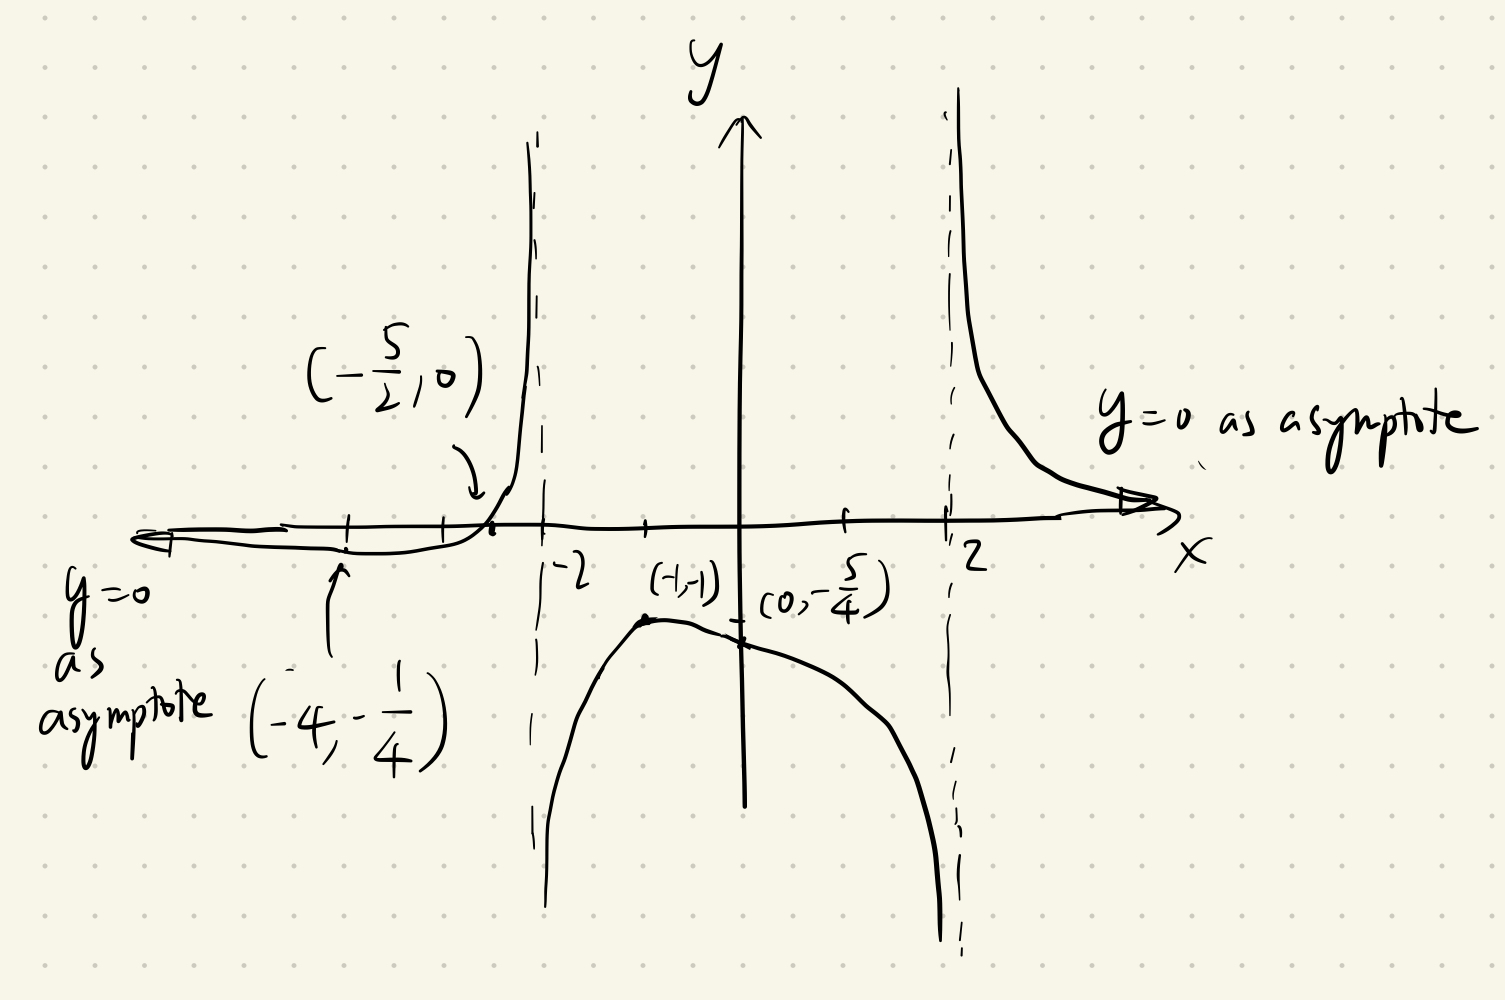
\includegraphics[width = 0.7\textwidth]{../graph/A12_Sol_4.png}
\end{figure}
\vspace{6mm}

% \problem Use the hinted linear approximations to approximate the following quantities:
% \begin{enumerate}[(a)]
%     \item $\tan 46 \degree$, approximating $\tan x$ at $x = 45 \degree$. (Note: You'll have to operate in radians) 
%     \item $\ln(1.01)$, approximating $\ln (1+x)$ at $x = 0$.
%     \item $\tan^{-1}0.99$, approximating $\tan^{-1} x$ at $x = 1$.
%     \item $\sqrt[4]{80}$, approximating $3\sqrt[4]{1+x}$ at $x = 0$.
%     \item $\frac{1}{0.99^3}$, approximating $\frac{1}{(1+x)^3}$ at $x = 0$.
% \end{enumerate}\vspace{6mm}

% \problem Find the following limits. You \textit{may} use the L'Hôpital's rule \textit{if applicable}.
% \begin{enumerate}[(a)]
%     \item $\lim\limits_{x \to 1} \frac{x^3+x^2+x-3}{x^3+2x^2+x-3}$
%     \item $\lim\limits_{x \to 0} \frac{e^{(3x^2+2x)}-1}{\sin(2x^2+3x)}$
%     \item $\lim\limits_{x \to 0} \frac{\sin (x^2)}{x \tan x}$
%     \item $\lim\limits_{x \to 0} x^2 \ln (x^2)$ \quad (Hint: Transform it into $\frac{\infty}{\infty}$ form)
%     \item $\lim\limits_{x \to 0} \frac{e^{-\frac{1}{x^2}}}{x^2}$ \quad (Hint: $\frac{0}{0}$ form can also be transformed into $\frac{\infty}{\infty}$ form)
% \end{enumerate}\vspace{4mm}

% \problem Determine if the following statements are true or false and explain. (You can just provide a counterexample if you determine them as false)
% \begin{enumerate}[(a)]
%     \item If $f'(x) = g'(x)$ (for all $x\in \mathbb{R}$), then $f(x) = g(x)$
%     \item If $f(1) = 0$, then $f'(1) = 0$
%     \item If $f'(x) = 0$ (for all $x\in \mathbb{R}$), then $f(x) = 0$
% \end{enumerate}\vspace{6mm}

% \problem Let $f(x) = \sqrt[4]{x} - \sqrt{x}$,
% \begin{enumerate}[(a)]
%     \item Find the tangent line of $f(x)$ at the point where $x=16$.
%     \item At which point(s) on $f(x)$ is its tangent line horizontal?
%     \item Is $f(x)$ differentiable at $x = 0$? Why?
% \end{enumerate}\vspace{6mm}

% \problem A ball is expanding with its radius $r$ as a function of time $t$: $r(t) = \sqrt{t} + 2, t \ge 0$
% \begin{enumerate}[(a)]
%     \item Find the rate its radius is growing at $t = 1$
%     \item Find the rate its surface area is growing at $t = 1$
%     \item Find the rate its volume is growing at $t = 1$
% \end{enumerate}\vspace{6mm}

\end{document}